\documentclass[border=12pt]{standalone}
\usepackage{tikz}
\usepackage{amsmath,amssymb}
\usetikzlibrary{calc,decorations.pathreplacing,arrows.meta}
\begin{document}
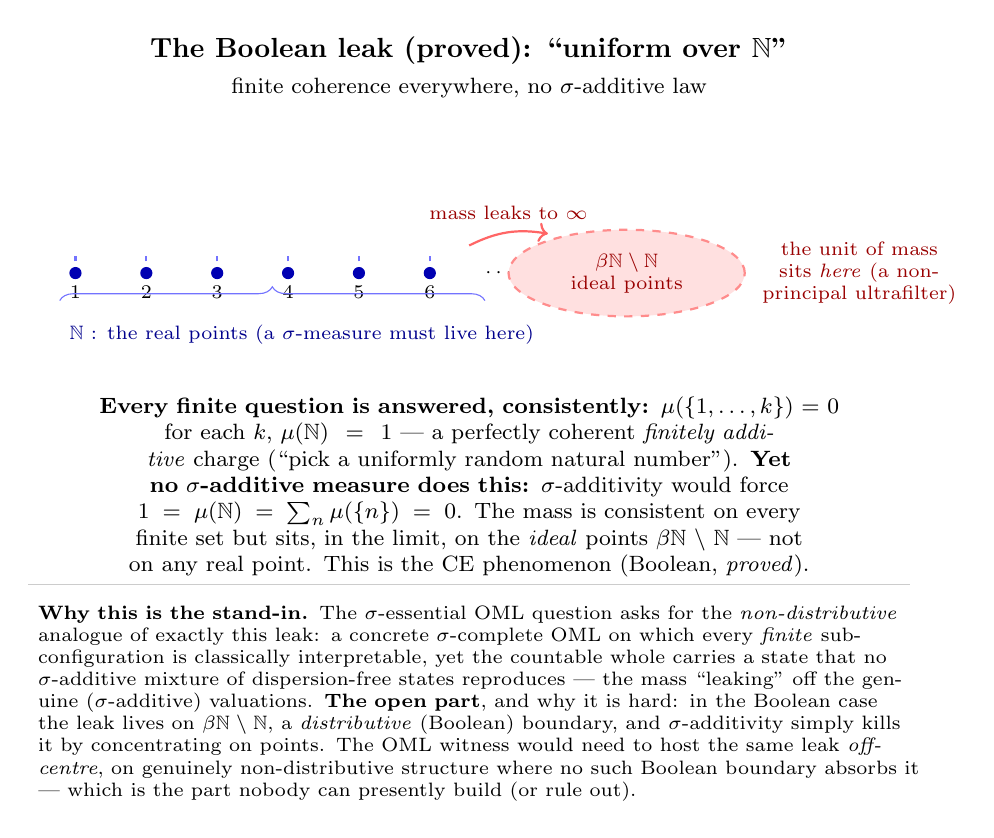
\begin{tikzpicture}[scale=1.0]

% =====================================================================
% The Boolean CE leak: a PROVED stand-in for the sigma-essential mechanism.
% "Uniform over N": every finite question is consistent and answerable, but the
% limit is only finitely additive -- mass leaks off the real points to the
% ideal points (non-principal ultrafilters, the boundary of the Stone space).
% =====================================================================

\node[anchor=south,align=center] at (5,3.5)
  {\textbf{The Boolean leak (proved): ``uniform over $\mathbb N$''}\\[1pt]
   \footnotesize finite coherence everywhere, no $\sigma$-additive law};

% ---- the real points: N, with uniform-on-prefix weights shrinking to 0 ----
\foreach \n/\x in {1/0.0,2/0.9,3/1.8,4/2.7,5/3.6,6/4.5}{
  \fill[blue!70!black] (\x,1.4) circle (2.2pt);
  \node[font=\scriptsize,below=1pt] at (\x,1.4) {$\n$};}
\node[font=\scriptsize] at (5.4,1.4){$\cdots$};
% bars over each point: "prob of {n} = 0" under the uniform-over-N charge
\foreach \x in {0.0,0.9,1.8,2.7,3.6,4.5}{
  \draw[blue!55,thick] (\x,1.55)--(\x,1.62);}  % vanishing weight
\node[blue!55!black,font=\scriptsize,anchor=west] at (6.0,1.4)
  {each $\mu(\{n\})=0$};

% ---- the bracket: N = the real (principal) points ----
\draw[decorate,decoration={brace,amplitude=5pt},blue!55] (-0.2,1.05)--(5.2,1.05);
\node[blue!55!black,font=\scriptsize,anchor=west] at (-0.2,0.62){$\mathbb N$ : the real points (a $\sigma$-measure must live here)};

% ---- the ideal boundary: where the mass actually goes ----
\fill[red!12] (7.0,1.4) ellipse (1.5 and 0.55);
\draw[red!45,thick,dashed] (7.0,1.4) ellipse (1.5 and 0.55);
\node[red!60!black,font=\scriptsize,align=center] at (7.0,1.4)
  {$\beta\mathbb N\setminus\mathbb N$\\ideal points};
\node[red!60!black,font=\scriptsize,align=center,anchor=west] at (8.6,1.4)
  {the unit of mass\\sits \emph{here} (a non-\\principal ultrafilter)};

% ---- the "leak" arrow: mass flows from N off to the boundary ----
\draw[->,red!60,thick] (5.0,1.75) to[bend left=18] (6.0,1.9);
\node[red!60!black,font=\scriptsize,anchor=south] at (5.5,1.95){mass leaks to $\infty$};

% ---- the finite-vs-sigma statement ----
\node[anchor=north,align=center,font=\footnotesize,text width=9.6cm] at (5,-0.05)
  {\textbf{Every finite question is answered, consistently:}
   $\mu(\{1,\dots,k\})=0$ for each $k$, $\mu(\mathbb N)=1$ --- a perfectly coherent
   \emph{finitely additive} charge (``pick a uniformly random natural number'').
   \textbf{Yet no $\sigma$-additive measure does this:} $\sigma$-additivity would force
   $1=\mu(\mathbb N)=\sum_n\mu(\{n\})=0$. The mass is consistent on every finite set but
   sits, in the limit, on the \emph{ideal} points $\beta\mathbb N\setminus\mathbb N$ ---
   not on any real point. This is the CE phenomenon (Boolean, \emph{proved}).};

% ---- the bridge line to the open problem ----
\draw[gray!40] (-0.6,-2.55)--(10.6,-2.55);
\node[anchor=north west,align=left,font=\scriptsize,text width=11.2cm] at (-0.6,-2.7)
  {\textbf{Why this is the stand-in.} The $\sigma$-essential OML question asks for the
   \emph{non-distributive} analogue of exactly this leak: a concrete $\sigma$-complete
   OML on which every \emph{finite} sub-configuration is classically interpretable, yet
   the countable whole carries a state that no $\sigma$-additive mixture of
   dispersion-free states reproduces --- the mass ``leaking'' off the genuine
   ($\sigma$-additive) valuations. \textbf{The open part}, and why it is hard: in the
   Boolean case the leak lives on $\beta\mathbb N\setminus\mathbb N$, a \emph{distributive}
   (Boolean) boundary, and $\sigma$-additivity simply kills it by concentrating on
   points. The OML witness would need to host the same leak \emph{off-centre}, on
   genuinely non-distributive structure where no such Boolean boundary absorbs it ---
   which is the part nobody can presently build (or rule out).};

\end{tikzpicture}
\end{document}
